\chapter{\ResearchTwoTitle}
\label{rq2:chapter}

本章研究通信预算受限下的多无人机语义消息选择方法。在单次观测任务中，允许传输的词元总量有限，而多架无人机针对局部画面生成的语义消息既可能相互重复，也可能因视角受遮挡而产生误判。为了在有限预算下提高地面中心的分类准确率，本章结合地面中心当前掌握的信息与无线链路状态，筛选对最终分类有补充作用的内容，并逐步确定待发消息的来源节点、详略程度以及停止发送的时机。

如图~\ref{rq2:fig:observation} 所示，多架无人机对同一目标区域的局部观测往往既存在视角互补，也难免出现区域重叠，且不同表达粒度对应的消息长度差异显著。地面中心需要结合已汇集的证据，有针对性地挑选后续增量内容。

\begin{figure}[htbp]
\centering
% Conceptual multi-view communication scene, not an experimental image.
% The receiver has no image observation. Labels denote candidate message
% granularities, not ground-truth visibility classes or scheduled decisions.
\begin{tikzpicture}[
  x=1mm,y=1mm,>=Stealth,
  font=\fontsize{9bp}{11.5bp}\selectfont,
  osnote/.style={align=center,fill=white,inner sep=.5mm},
  osray/.style={line width=.4pt,dash pattern=on 2pt off 1.5pt},
  oslink/.style={->,line width=.65pt},
  pics/osdrone/.style args={#1}{code={
    \draw[line width=.65pt,draw=black!80] (-3.4,-1.6)--(3.4,1.6)
      (-3.4,1.6)--(3.4,-1.6);
    \foreach \px/\py in {-4.1/-1.9,-4.1/1.9,4.1/-1.9,4.1/1.9}
      \draw[line width=.55pt,draw=black!80,fill=white]
        (\px,\py) ellipse[x radius=1.8mm,y radius=.65mm];
    \draw[line width=.55pt,draw=black!80,fill=#1!18]
      (0,0) ellipse[x radius=1.4mm,y radius=.9mm];
    \draw[line width=.45pt,draw=black!80] (-.75,-.7)--(-.75,-1.5)
      (.75,-.7)--(.75,-1.5);
    \draw[line width=.4pt,draw=black!80,fill=white]
      (-.5,-1.7) rectangle (.5,-2.4);
  }}
]
\definecolor{osblue}{RGB}{66,104,135}
\definecolor{osgreen}{RGB}{84,123,99}
\definecolor{osorange}{RGB}{177,130,76}
\path[use as bounding box] (0,0) rectangle (148,90);

% Shared ground plane and a road in oblique projection.
\filldraw[fill=black!2,draw=black!35,line width=.45pt]
  (4,9)--(119,9)--(144,35)--(29,35)--cycle;
\filldraw[fill=black!9,draw=black!35,line width=.45pt]
  (14,19)--(129,19)--(135,25)--(20,25)--cycle;
\draw[white,line width=.8pt,dash pattern=on 3mm off 2mm]
  (17,22)--(132,22);

% Light view pyramids and overlapping footprints. A and C see much of the
% same region; B extends coverage to the right of the occluding structure.
\fill[osblue,opacity=.035] (24,54.6)--(8,12)--(53,12)--(71,31)--cycle;
\fill[osorange,opacity=.035] (61,56.6)--(29,13)--(74,13)--(93,32)--cycle;
\fill[osgreen,opacity=.035] (103,54.6)--(74,10)--(119,10)--(141,32)--cycle;
\filldraw[fill=osblue,fill opacity=.10,draw=osblue!85,line width=.55pt]
  (8,12)--(53,12)--(71,31)--(26,31)--cycle;
\filldraw[fill=osorange,fill opacity=.10,draw=osorange!90,line width=.55pt]
  (29,13)--(74,13)--(93,32)--(48,32)--cycle;
\filldraw[fill=osgreen,fill opacity=.10,draw=osgreen!85,line width=.55pt]
  (74,10)--(119,10)--(141,32)--(95,32)--cycle;
\foreach \p in {(8,12),(53,12),(71,31),(26,31)}
  \draw[osray,osblue!65] (24,54.6)--\p;
\foreach \p in {(29,13),(74,13),(93,32),(48,32)}
  \draw[osray,osorange!70] (61,56.6)--\p;
\foreach \p in {(74,10),(119,10),(141,32),(95,32)}
  \draw[osray,osgreen!65] (103,54.6)--\p;

% A low structure creates a region hidden from some viewing directions.
\fill[black!12] (68,18)--(87,18)--(94,25)--(76,25)--cycle;
\draw[black!40,line width=.35pt,densely dashed]
  (76,18)--(87,18)--(94,25);
\filldraw[fill=black!13,draw=black!60,line width=.45pt]
  (58,23)--(73,23)--(73,34)--(58,34)--cycle;
\filldraw[fill=black!20,draw=black!60,line width=.45pt]
  (73,23)--(82,32)--(82,43)--(73,34)--cycle;
\filldraw[fill=black!5,draw=black!60,line width=.45pt]
  (58,34)--(73,34)--(82,43)--(67,43)--cycle;
\node[osnote,inner sep=.25mm] at (65.5,28.5) {遮挡物};
\node[osnote,inner sep=.25mm] (osoccluded) at (87,6.3) {部分视角受遮挡};
\draw[black!55,line width=.4pt] (osoccluded.north)--(84,18.5);
\node[fill=white,inner sep=.25mm] at (108,23) {道路};
\node[fill=white,inner sep=.25mm] at (34,8.1) {共同地面观测区域};

% Line-drawn quadrotors retain a small size relative to their footprints.
\pic at (24,57) {osdrone=osblue};
\pic at (61,59) {osdrone=osorange};
\pic at (103,57) {osdrone=osgreen};
\node[osnote,text=osblue!90!black] at (24,48.5) {视角 A：局部可见};
\node[osnote,text=osorange!90!black] at (61,50.5) {视角 C：重叠观测};
\node[osnote,text=osgreen!90!black] at (108,46.5) {视角 B：补充区域};

% Candidate semantic messages, with illustrative (unmeasured) payload sizes.
\draw[oslink,osblue] (25,60.2)
  .. controls (43,83) and (102,86) .. (129.5,75);
\draw[oslink,osorange] (63,62)
  .. controls (86,78) and (111,77) .. (129.5,73.2);
\draw[oslink,osgreen] (105,60)
  .. controls (116,61) and (126,67) .. (129.5,71.5);
\filldraw[fill=white,draw=osblue,line width=.45pt]
  (59,75.8) rectangle (71,83.8);
\node[text=osblue!90!black] at (65,80.5) {标签};
\draw[osblue,line width=.6pt] (62.5,77.5)--(67.5,77.5);
\filldraw[fill=white,draw=osorange,line width=.45pt]
  (85,70.7) rectangle (105,78.7);
\node[text=osorange!90!black] at (95,75.5) {陈述};
\draw[osorange,line width=.6pt] (89,72.5)--(101,72.5);
\filldraw[fill=white,draw=osgreen,line width=.45pt]
  (102,60.2) rectangle (126,69.2);
\node[text=osgreen!90!black] at (114,66.2) {摘要};
\draw[osgreen,line width=.55pt] (105,63.5)--(123,63.5)
  (105,61.8)--(119,61.8);

% Blind receiver: a monitor and antenna, not another image sensor.
\draw[fill=white,draw=black!80,line width=.6pt]
  (130,68.5) rectangle (138,75);
\draw[black!55,line width=.35pt] (131,70)--(137,70);
\draw[black!80,line width=.6pt] (134,68.5)--(134,66.4)
  (130.7,66.4)--(137.3,66.4);
\draw[black!75,line width=.5pt] (140,70)--(140,76);
\draw[black!65,line width=.45pt] (141.1,74.9) arc[start angle=-40,end angle=40,radius=1.6mm]
  (142.2,74.1) arc[start angle=-40,end angle=40,radius=3mm];
\node[osnote,text width=25mm] at (134,83.6) {接收中心\\不读取原图};

\node[align=center] at (74,1.8)
  {虚线：局部视野\qquad 实线箭头：候选语义消息};
\end{tikzpicture}

\bicaption{多视角观测与多粒度语义证据选择示意}{Multi-view observation and multi-granularity semantic evidence selection}
\label{rq2:fig:observation}
\end{figure}

为此，本章提出基于强化学习的语义消息选择方法 EviComRL。该方法先由参数冻结的视觉语言模型针对各局部视角生成不同详略程度的候选消息，再由选择策略结合节点观测可靠性、地面中心当前判断、已选消息记录和链路开销，评估各条候选的发送价值。决策时通过动作掩码排除重复发送和超出词元预算的选项，并采用 PPO 算法优化策略参数。最后，本章通过实验评估了 EviComRL 在不同词元预算、链路条件及视角数量下的分类准确率与通信开销。

\section{系统模型与问题描述}
\label{rq2:sec:model}

\subsection{观测任务与消息表示}

考虑包含 $N$ 个局部观测节点（记为集合 $\mathcal N=\{1,\ldots,N\}$）和一个决策中心 $c_0$ 的协同观测系统。第 $k$ 项任务由完整场景图像 $I_k$ 与自然语言查询 $q_k$ 定义，每架无人机仅能观测到局部裁剪区域 $o_{i,k}$，以此模拟受限视场及视角覆盖差异；底层视觉语言模型在整个研究过程中保持参数冻结。

借助 VQAv2 数据集的视觉问答对与 COCO 图像\cite{vqa-v2,coco}，本文构造了面向查询的证据可见性判别任务，用于评估局部画面能否为回答给定问题提供充分依据。类别空间定义为五级离散标签：
\begin{equation}
\mathcal Y=\{\text{清晰可见},\text{大部分可见},\text{不确定},\text{大部分遮挡},\text{完全遮挡}\}.
\label{rq2:eq:labels}
\end{equation}
实验按标准五分类任务进行训练与评估。这里的“可见性”并非简单指目标是否出现在画面中，而是指局部画面是否包含足以回答特定属性或关系问题的有效证据，不同查询往往对应图像中的不同关注区域\cite{where-to-look-vqa,vqa-hat,gqa}。训练与离线评估所需的弱监督参考标签 $y_k^*$ 由冻结模型依据完整图像与查询直接生成（不作为策略输入），各局部节点仅根据自身裁剪图提取证据。因此，本章分类准确率刻画的是经多机通信融合后的中心判断与全图参考判断之间的一致性。

节点 $i$ 从局部观测 $o_{i,k}$ 中提取的证据表示为七元组：
\begin{equation}
e_{i,k}=\left(y_{i,k},p_{i,k},u_{i,k},q_{i,k}^{\mathrm{obs}},\ell_{i,k},r_{i,k},\bm b_{i,k}\right),
\label{rq2:eq:evidence}
\end{equation}
依次对应局部预测标签、置信度、不确定性、观测质量评分、裁剪区域坐标、文本摘要以及五维语义信念向量 $\bm b_{i,k}\in\mathbb R^5$（满足 $b_{i,k}^{y}\geq0$ 且 $\sum_y b_{i,k}^{y}=1$）。节点局部信念的香农熵为
\begin{equation}
H(\bm b_{i,k})=-\sum_{y\in\mathcal Y}b_{i,k}^{y}\log\max\{b_{i,k}^{y},\varepsilon\}.
\label{rq2:eq:entropy}
\end{equation}
其中置信度、熵和观测质量分别反映预测的集中程度、分布不确定性以及画面本身的清晰完整程度。需要注意的是，严重遮挡的低质量视角同样可能输出高置信度的错误判断，因此仅凭单一置信度难以挑选可靠证据，必须横向比对不同节点的观测质量与判断结论。

在基准配置下，地面中心初始时没有本地观测画面，因此将初始信念设为均匀分布 $\bm b_{c_0,k}^{0}=\bm u=(1/5,\ldots,1/5)$。未被选中节点的局部信念只用于构造选择阶段的候选特征，不会参与地面中心的最终分类。这部分信息仅作调度参考，本身数据量很小，不计入语义消息的词元预算。

针对同一份局部证据，按详略程度构造四种表达粒度（消息模式）：
\begin{equation}
\mathcal C=\{\mathrm{label},\mathrm{claim},\mathrm{summary},\mathrm{full}\},
\label{rq2:eq:modes}
\end{equation}
依次携带类别标签、核心判断陈述、附带依据的摘要以及完整结构化证据。每条候选消息记为 $m=(i,j,c)$，对应发送节点、接收节点及消息模式，其词元长度为 $T_m$。显然，同一节点的不同模式共享底层观测视角，重复选用虽可能强化原有结论，却会挤占引入其他互补视角的预算。在一般节点间定向通信下，候选空间至多为 $N(N-1)|\mathcal C|$；在盲中心基准配置下，所有消息均发往中心 $c_0$，候选退化为“发送方--模式”组合（规模约 $N|\mathcal C|$），核心决策即在于序贯选择消息来源、表达粒度以及停止时机。

为刻画底层无线链路对上层消息选择的影响，设节点 $i,j$ 间距为 $d_{ij}$，带宽状态因子与链路质量因子分别为 $\eta_{ij}^{\mathrm{bw}}$ 和 $\eta_{ij}^{\mathrm{link}}$，采用如下距离与信道感知的有效传输速率模型：
\begin{equation}
v_{ij}=\left(v_{\max}e^{-\zeta d_{ij}}+v_{\min}\right)
\max\{0.05,\eta_{ij}^{\mathrm{bw}}\eta_{ij}^{\mathrm{link}}\}.
\label{rq2:eq:rate}
\end{equation}
记单个 token 对应的平均字节数为 $b_{\mathrm{tok}}$，则消息字节大小 $B_m$、发送时延 $L_m$ 与发射能耗 $E_m$ 分别为
\begin{equation}
B_m=b_{\mathrm{tok}}T_m,\qquad
L_m=\frac{B_m}{v_{ij}},\qquad E_m=P_{\mathrm{tx}}L_m.
\label{rq2:eq:cost}
\end{equation}
进一步设当前链路的可用接触窗口为 $D_m$，以平滑逻辑函数刻画消息在窗口内成功送达的概率及对应丢包风险：
\begin{equation}
p_m^{\mathrm{del}}=\frac{1}{1+\exp[-(D_m-L_m)/\tau]},\qquad
R_m^{\mathrm{drop}}=1-p_m^{\mathrm{del}},
\label{rq2:eq:delivery}
\end{equation}
其中，温度参数 $\tau$ 用于调节送达概率在窗口边界附近的变化快慢。消息越长，单次发送耗时越久，越容易因超出传输窗口而丢包；带宽越宽、链路质量越好，发送耗时相应缩短，消息成功送达的概率也就越高。

\subsection{观测数据与优化目标}

实验中提前离线生成并保存全部任务的观测数据，包括参考标签、各节点局部证据、消息代价及对应的信念更新量。这样既能保证不同通信策略在相同数据下对比，也能避免训练过程中反复在线调用视觉语言模型带来的计算开销和输出波动。对于节点间传输的单条消息，由参数冻结的语义更新模块 $\mathcal U$ 给出的信念增量为
\begin{equation}
\Delta\bm b_{i\to j,k}^{c}
=\kappa_c\left[\mathcal U(o_{j,k},e_{j,k},m_{i\to j,k}^{c})-\bm b_{j,k}^{0}\right],
\label{rq2:eq:raw_update}
\end{equation}
其中 $\kappa_c$ 为不同粒度的融合权重。对于无初始观测的盲中心，基准配置将各模式对中心的信念增量统一定义为
\begin{equation}
\begin{aligned}
\Delta\bm b_{i\to c_0,k}^{c}&=\kappa_c(\bm b_{i,k}-\bm u),\\
(\kappa_{\mathrm{label}},\kappa_{\mathrm{claim}},\kappa_{\mathrm{summary}},\kappa_{\mathrm{full}})
&=(0.22,0.42,0.62,0.78).
\end{aligned}
\label{rq2:eq:center_update}
\end{equation}
每当第 $t$ 步选中消息 $m_t$ 时，接收方按送达概率折扣后的增量更新语义信念：
\begin{equation}
\bm b_j^{t+1}=\mathcal P\!\left[\bm b_j^t+
\left(p_{m_t}^{\mathrm{del}}\right)^\alpha\Delta\bm b_{m_t}\right],
\label{rq2:eq:belief_update}
\end{equation}
其中，投影算子 $\mathcal P$ 将向量中的负分量置零并重新归一化；若所有分量均不大于零，则将其重置为均匀分布。基准实验取 $\alpha=0.5$，即按送达概率的平方根对信念增量进行折扣；后续消融实验还将对比 $\alpha=0$ 时不作折扣的情况。由于本章主要研究内容筛选策略本身，上述状态更新直接按期望折扣在离线数据上计算确定性的融合结果，不在每次发送时对单条消息是否丢包做随机抽样。即便如此，受非负截断与归一化运算的非线性影响，同一条候选消息在地面中心处于不同信念状态时，或按不同先后顺序被选中时，对最终分类结果带来的实际增益仍然不同。

\begin{figure}[htbp]
\centering
\begin{tikzpicture}[x=1mm,y=1mm,>=Stealth,
  font=\fontsize{9bp}{11.5bp}\selectfont,
  ewbox/.style={draw,line width=.45pt,align=center,text width=38mm,
    minimum height=10mm,inner sep=1mm},
  ewarrow/.style={->,line width=.55pt},
  ewnote/.style={align=center,inner sep=.4mm,fill=white}]
\path[use as bounding box] (0,1) rectangle (148,-42);
\node[ewnote] at (74,-1) {离线构造：参考标签仅用于训练与评价};
\node[ewbox] (image) at (25,-9.5) {完整图像与查询\\局部视角裁剪};
\node[ewbox] (vlm) at (74,-9.5) {参数固定的视觉语言模型\\标签、信念与摘要};
\node[ewbox] (trace) at (123,-9.5) {预先生成的观测数据\\消息、代价与增量};
\node[ewbox] (candidate) at (123,-25.5) {按质量与代价筛选\\更新候选排序};
\node[ewbox] (policy) at (74,-25.5) {来源质量与选择历史\\掩码策略网络};
\node[ewbox] (action) at (25,-25.5) {发送消息或停止\\中心信念与资源更新};
\draw[ewarrow] (image) -- (vlm);
\draw[ewarrow] (vlm) -- (trace);
\draw[ewarrow] (trace) -- (candidate);
\draw[ewarrow] (candidate) -- (policy);
\draw[ewarrow] (policy) -- (action);
\draw[ewarrow] (action.south) -- (25,-34.5) -- (74,-34.5) -- (policy.south);
\node[ewnote] at (49.5,-34.5) {当前判断、历史与预算};
\node[ewnote] at (74,-40) {训练：策略预训练与 PPO\qquad 测试：固定参数执行};
\end{tikzpicture}

\bicaption{观测数据生成与消息选择流程}{Observation data generation and message selection}
\label{rq2:fig:workflow}
\end{figure}

记第 $t$ 步前已选消息集合为 $\mathcal S_t$，累计消耗的词元数为 $U_t=\sum_{m\in\mathcal S_t}T_m$，接收方 $j$ 已收消息数为 $n_j^t$，发送方 $i$ 的剩余能量为 $e_i^t$。在总通信预算 $T_{\mathrm{bud}}$、最大决策步数 $H$、接收容量上限 $C_j$ 以及最低送达概率 $p_{\min}$ 与最低电量 $e_{\min}$ 约束下，任意合法候选消息 $m$ 须同时满足
\begin{equation}
\begin{aligned}
m&\notin\mathcal S_t, & U_t+T_m&\leq T_{\mathrm{bud}},\\
p_m^{\mathrm{del}}&\geq p_{\min}, & n_j^t&<C_j,\\
e_i^t&\geq e_{\min}, & t&<H.
\end{aligned}
\label{rq2:eq:constraints}
\end{equation}
发送后发送方电量更新为 $e_i^{t+1}=\max\{0,e_i^t-E_m\}$。

记实际停止步数为 $\tau_k\leq H$，则中心最终的类别预测与参考类别上的信念质量分别为
\begin{equation}
\hat y_k=\arg\max_{y\in\mathcal Y} b_{c_0,k}^{\tau_k,y},\qquad
Q_k= b_{c_0,k}^{\tau_k,y_k^*}.
\label{rq2:eq:quality}
\end{equation}
语义消息选择的整体目标是在可行域内学习策略 $\pi$，最大化最终任务判断质量与综合通信代价的加权差值：
\begin{equation}
\max_{\pi}\ \mathbb E_{k,\pi}\!\left[
\begin{aligned}
&\lambda_Q Q_k+\lambda_A\mathbf1\{\hat y_k=y_k^*\}
-\beta_T\frac{U_{\tau_k}}{T_{\mathrm{bud}}}\\
&\hspace{1em}-\beta_L\sum_{m\in\mathcal S_{\tau_k}}L_m
-\beta_R\sum_{m\in\mathcal S_{\tau_k}}R_m^{\mathrm{drop}}
\end{aligned}\right].
\label{rq2:eq:objective}
\end{equation}
由于信念融合具有非线性且子集规模与排序均可变，暴力枚举的组合复杂度极高。为此，EviComRL 先通过轻量级初筛压缩候选规模，再利用深度强化学习在线决策发送顺序与停止时机。

\section{语义消息选择方法}
\label{rq2:sec:algorithm}

\subsection{候选筛选与策略输入}

为控制强化学习的动作空间维度，EviComRL 首先在回合初始化阶段执行两级成本敏感筛选。记 $C_{ij}^{\mathrm{conf}}$ 为收发双方初始预测的冲突度，$C_{ij}^{\mathrm{comp}}$ 为基于视角重叠度计算的观测互补性，$b_c$ 为与表达粒度相关的强度项，初筛打分公式定义为
\begin{equation}
S_1(m)=\frac{H(\bm b_j^0)+C_{ij}^{\mathrm{conf}}+C_{ij}^{\mathrm{comp}}+q_i^{\mathrm{obs}}+0.2b_c}
{(T_m/T_{\mathrm{bud}}+L_m+\varepsilon)(1+R_m^{\mathrm{drop}})}.
\label{rq2:eq:retrieval}
\end{equation}
其中，分子综合反映接收端当前判断的不确定程度与发送端局部观测的质量，分母计入消息词元占比、传输时延和丢包风险，各项数值均由通信前已知的节点与链路状态直接算得。

取初筛排名前 $K$ 的候选，进一步按语义价值与链路条件的线性加权得分重排序：
\begin{equation}
\begin{aligned}
S_2(m)={}&H(\bm b_j^0)+C_{ij}^{\mathrm{conf}}+C_{ij}^{\mathrm{comp}}+q_i^{\mathrm{obs}}
+0.6\mathbf1\{j=c_0\}\\
&+0.4p_m^{\mathrm{del}}+0.2\eta_{ij}^{\mathrm{link}}+0.1\eta_{ij}^{\mathrm{bw}}
-0.7T_m/T_{\mathrm{bud}}-0.2L_m-0.4R_m^{\mathrm{drop}}.
\end{aligned}
\label{rq2:eq:rerank}
\end{equation}
截取排序靠前的前 $M$ 条消息作为当前回合的候选池，其中基准配置取 $K=32$、$M=16$。在后续逐步选择过程中，候选池不再引入新消息，仅在每步决策前根据最新信念状态和剩余预算更新候选特征与动作掩码。在所有消息均以地面中心 $c_0$ 为接收方的基准设定下，式~\eqref{rq2:eq:rerank} 中的中心偏好项为常数值，不会影响候选排序；只有当允许无人机之间相互转发消息时，该项才用来区分直接发往地面中心与先经其他节点中转这两类候选。

为弥补单条消息置信度易受局部遮挡误导的缺陷，本文为每个发送节点 $i$ 设计了五维可观测可靠性特征。将节点信念分量降序排列为 $b_i^{(1)}\geq b_i^{(2)}\geq\cdots$，构造
\begin{equation}
\begin{aligned}
\bm r_i&=[r_{i,1},r_{i,2},r_{i,3},r_{i,4},r_{i,5}],\\
r_{i,1}&=b_i^{(1)},\quad r_{i,2}=b_i^{(1)}-b_i^{(2)},\quad
r_{i,3}=H(\bm b_i)/\log5,\\
r_{i,4}&=\frac{\sum_{v\ne i}\mathbf1\{q_v^{\mathrm{obs}}<q_i^{\mathrm{obs}}\}}{\max(1,|\mathcal V|-1)},\quad
r_{i,5}=\frac{\sum_v q_v^{\mathrm{obs}}\mathbf1\{\hat y_v=\hat y_i\}}{\sum_v q_v^{\mathrm{obs}}+\varepsilon},
\end{aligned}
\label{rq2:eq:reliability}
\end{equation}
其中，集合 $\mathcal V$ 包含观测质量为零的地面中心。这五项分别表示最大预测概率、前两类概率差值、归一化不确定度、节点观测质量的相对排名，以及按观测质量加权的群体共识度。质量加权共识在多数情况下能够减弱低质量视角带来的干扰，但如果多数视角同时误判，该项也会引入偏差。

将上述特征拼接后，每条候选消息对应一个 41 维特征向量，具体构成见表~\ref{rq2:tab:features}。同时，构造 11 维全局状态向量 $\bm g_t$，包含剩余预算比例、地面中心最大信念值、当前步数占比、已耗预算占比、累计时延、累计能耗以及当前五维语义信念。这里的地面中心最大信念值直接由当前信念分布得到，用来反映可观测的置信度，不同于依赖参考标签计算的 $Q_k$。第 $t$ 步策略网络的状态输入记为 $s_t=(X_t,\bm g_t,\bm\mu_t)$，其中 $X_t\in\mathbb R^{M\times41}$ 为候选特征矩阵，$\bm\mu_t$ 为由式~\eqref{rq2:eq:constraints} 确定的动作掩码。

\begin{table}[htbp]
\centering
\bicaption{候选消息的结构化特征组成}{Structured features of each candidate message}
\label{rq2:tab:features}
\small
\setlength{\tabcolsep}{5pt}
\renewcommand{\arraystretch}{0.92}
\begin{tabularx}{\textwidth}{l r X}
\toprule
特征类别 & 维数 & 具体内容\\
\midrule
发送方与证据关系 & 6 & 置信度、不确定性、观测质量、接收方熵、预测冲突、观测互补性\\
语义粒度 & 4 & 四种消息模式的独热编码\\
通信与历史状态 & 10 & 消息长度、时延、窗口、送达概率、丢包风险、已选状态、中心标记、链路质量、带宽因子、能量代价\\
节点信念 & 15 & 发送方、接收方和决策中心各自的五维信念\\
可靠性信息 & 5 & 信念峰值、类别间隔、归一化熵、观测质量排名、加权共识\\
候选存在标记 & 1 & 区分真实候选与补齐固定长度的空白项\\
\bottomrule
\end{tabularx}
\end{table}

\subsection{消息选择策略网络}

EviComRL 的策略网络结构如图~\ref{rq2:fig:network} 所示。首先，基础编码器采用两层全连接网络处理候选特征，并与全局编码器一起将原始输入映射到 64 维隐藏空间，分别得到候选基础表示 $\bm h_m^0=f_{\mathrm{cand}}(\bm x_m)$ 和全局表示 $\bm z_t=f_g(\bm g_t)$。同时，网络设置 6 个并行的属性编码分支 $\bm v_m^a=f_a(\bm x_m^a)$，其中 $a\in\{s,r,c,l,b,q\}$，各分支均采用全连接层加 $\tanh$ 激活函数，分别编码发送方、接收方、语义模式、链路代价、三方信念和可靠性六类属性特征。上述基础编码器与各属性分支对所有候选消息共享参数。

考虑到已选消息会影响后续候选的选取，网络根据候选存在标记 $e_m$、已选标记 $s_m^t$ 和中心接收标记 $c_m$，对候选基础表示 $\bm h_m^0$ 分别求加权均值，得到已选历史上下文和中心上下文：
\begin{equation}
\bar{\bm h}_t^{\mathrm{sel}}=
\frac{\sum_m e_ms_m^t\bm h_m^0}{\max(1,\sum_m e_ms_m^t)},\qquad
\bar{\bm h}_t^{\mathrm{ctr}}=
\frac{\sum_m e_mc_m\bm h_m^0}{\max(1,\sum_m e_mc_m)}.
\label{rq2:eq:history}
\end{equation}
两者均随每步中心信念的刷新而实时更新。随后，将基础候选表示、六个结构分支输出、两类上下文向量及全局嵌入拼接，经融合层 $f_{\mathrm{rel}}$ 生成交互表征 $\bm u_m$，并通过门控残差机制与基础表示结合：
\begin{equation}
\bm a_m=\sigma\!\left(W_a[\bm h_m^0,\bm u_m,\bm z_t]+\bm b_a\right),\qquad
\bm h_m=\bm h_m^0+\bm a_m\odot\bm u_m.
\label{rq2:eq:gate}
\end{equation}
其中门控偏置 $\bm b_a$ 初始化为负值，使训练初期网络优先依赖稳定的基础编码，再逐步放开关系分支的残差修正，防止初期随机梯度引发策略震荡。

\begin{figure}[htbp]
\centering
% Matches GraphHistoryActorCriticNet and Eqs. (encoders)--(policy).
\begingroup
\begin{tikzpicture}[
  x=1mm,y=1mm,>=Stealth,
  font=\fontsize{8.2bp}{9.8bp}\selectfont,
  inframe/.style={draw=black!80,line width=.55pt,fill=blue!9!white,
    align=center,inner sep=1.2mm,outer sep=0pt},
  modbox/.style={draw=black!80,line width=.55pt,fill=black!2!white,
    align=center,inner sep=1.2mm,outer sep=0pt},
  ctxbox/.style={draw=blue!55!black,line width=.5pt,fill=blue!3!white,
    align=center,inner sep=1.1mm,outer sep=0pt},
  outbox/.style={draw=black!80,line width=.55pt,fill=white,
    align=center,inner sep=1.2mm,outer sep=0pt},
  headfill/.style={fill=blue!7!white},
  dataedge/.style={-{Stealth[length=1.5mm,width=1.05mm]},
    draw=black!85,line width=.6pt},
  datawire/.style={draw=black!85,line width=.6pt},
  ctxedge/.style={-{Stealth[length=1.5mm,width=1.05mm]},
    draw=blue!55!black,line width=.55pt},
  ctxwire/.style={draw=blue!55!black,line width=.55pt},
  maskedge/.style={-{Stealth[length=1.5mm,width=1.05mm]},
    draw=black!65,line width=.55pt,dashed,dash pattern=on 1.3mm off .8mm},
  halo/.style={preaction={draw=white,line width=2.2pt}},
  lbl/.style={font=\fontsize{7.8bp}{9bp}\selectfont,inner sep=.8pt}
]
\path[use as bounding box] (0,0) rectangle (148,-112);

% 第1层：外部输入（候选特征与全局状态相互独立）
\node[inframe,anchor=north west,minimum width=108mm,minimum height=7mm]
  (enx) at (0,0)
  {\textbf{候选特征输入}\ $X_t\in\mathbb R^{M\times 41}$};
\node[inframe,anchor=north west,minimum width=35mm,minimum height=7mm]
  (engin) at (113,0)
  {\textbf{全局状态}\ $\bm g_t\in\mathbb R^{11}$};

% 第2层：特征编码（将6路属性合并为一个分组编码模块）
\node[modbox,anchor=north west,minimum width=64mm,minimum height=14mm]
  (enattr) at (0,-12.5)
  {\textbf{分组属性编码（6路）}\\
   发送方 $\bm v_m^s$、接收方 $\bm v_m^r$、语义模式 $\bm v_m^c$\\
   链路代价 $\bm v_m^l$、三方信念 $\bm v_m^b$、可靠性 $\bm v_m^q$};
\node[modbox,anchor=north west,minimum width=39mm,minimum height=14mm]
  (enbase) at (69,-12.5)
  {\textbf{基础编码}\\
   候选基础表示 $\bm h_m^0$};
\node[ctxbox,anchor=north west,minimum width=35mm,minimum height=14mm]
  (englob) at (113,-12.5)
  {\textbf{全局编码} $f_g$\\
   全局表示 $\bm z_t$};

\draw[dataedge] (32,-7) -- (32,-12.5);
\draw[dataedge] (88.5,-7) -- (88.5,-12.5);
\draw[ctxedge]  (130.5,-7) -- (130.5,-12.5);

% 第3层：上下文池化（仅对基础表示 h_m^0 加权池化）
\node[ctxbox,anchor=north west,minimum width=29mm,minimum height=11mm]
  (ensel) at (64,-32.5)
  {已选历史 $\bar{\bm h}_t^{\mathrm{sel}}$\\
   按 $e_m s_m^t$ 池化};
\node[ctxbox,anchor=north west,minimum width=29mm,minimum height=11mm]
  (enctr) at (96,-32.5)
  {中心上下文 $\bar{\bm h}_t^{\mathrm{ctr}}$\\
   按 $e_m c_m$ 池化};

% 基础编码输出分流：两路进上下文池化，一路向下进关系编码与门控残差
\draw[datawire] (88.5,-26.5) -- (88.5,-29.5);
\draw[datawire] (56,-29.5) -- (110.5,-29.5);
\fill[black!85] (88.5,-29.5) circle (.4mm);
\fill[black!85] (78.5,-29.5) circle (.4mm);
\draw[dataedge] (78.5,-29.5) -- (78.5,-32.5);
\draw[dataedge] (110.5,-29.5) -- (110.5,-32.5);

% 全局编码输出分流：一路进右侧共享上下文总线，一路向下进门控残差
\draw[ctxwire] (130.5,-26.5) -- (130.5,-29.5) -- (143,-29.5);
\fill[blue!55!black] (130.5,-29.5) circle (.4mm);

% 共享上下文总线（汇聚已选历史、中心上下文与全局表示）
\draw[ctxwire] (78.5,-43.5) -- (78.5,-46.5);
\draw[ctxwire] (110.5,-43.5) -- (110.5,-46.5);
\draw[ctxwire] (143,-29.5) -- (143,-73.5);
\draw[ctxwire] (50,-46.5) -- (143,-46.5);
\fill[blue!55!black] (78.5,-46.5) circle (.4mm);
\fill[blue!55!black] (110.5,-46.5) circle (.4mm);
\fill[blue!55!black] (143,-46.5) circle (.4mm);
\draw[ctxedge] (50,-46.5) -- (50,-53.5);

% 第4层：关系编码与门控残差融合
\node[modbox,anchor=north west,minimum width=60mm,minimum height=12mm]
  (enrel) at (0,-53.5)
  {\textbf{关系编码} $f_{\mathrm{rel}}$\\
   融合基础、属性与上下文，输出 $\bm u_m$};
\node[modbox,anchor=north west,minimum width=64mm,minimum height=12mm]
  (engate) at (72,-53.5)
  {\textbf{门控残差融合}\\
   $\bm h_m=\bm h_m^0+\bm a_m\odot\bm u_m$};

% 6路属性直连关系编码
\draw[dataedge] (22,-26.5) -- (22,-53.5);
\node[lbl,anchor=west] at (23.2,-38) {$\bm v_m^*$};

% h_m^0 连入关系编码，并作为残差跳连进入门控融合
\draw[datawire,halo] (56,-29.5) -- (56,-50);
\draw[datawire] (36,-50) -- (88,-50);
\fill[black!85] (56,-50) circle (.4mm);
\draw[dataedge] (36,-50) -- (36,-53.5);
\draw[dataedge] (88,-50) -- (88,-53.5);
\node[lbl,anchor=east] at (54.8,-38) {$\bm h_m^0$};

% z_t 连入门控残差融合（控制门控系数 a_m）
\draw[ctxedge,halo] (130.5,-29.5) -- (130.5,-53.5);
\node[lbl,anchor=west,text=blue!55!black] at (131.7,-38) {$\bm z_t$};

% 关系编码 -> 门控残差融合
\draw[dataedge] (60,-59.5) -- (72,-59.5);
\node[lbl,anchor=south] at (66,-58.8) {$\bm u_m$};

% 第5层：策略网络与价值网络
\fill[headfill] (0,-77) rectangle (64,-82.2);
\draw[black!60,line width=.4pt] (0,-82.2) -- (64,-82.2);
\draw[black!80,line width=.55pt] (0,-77) rectangle (64,-94);
\node[align=center,inner sep=0pt] at (32,-79.6) {\textbf{策略网络}};
\node[align=center,text width=61mm,inner sep=0pt] at (32,-88.1)
  {消息头：由 $\bm h_m$ 与上下文输出 $\ell_m$\\
   停止头：由上下文输出 $\ell_0$};

\fill[headfill] (74,-77) rectangle (136,-82.2);
\draw[black!60,line width=.4pt] (74,-82.2) -- (136,-82.2);
\draw[black!80,line width=.55pt] (74,-77) rectangle (136,-94);
\node[align=center,inner sep=0pt] at (105,-79.6) {\textbf{价值网络}};
\node[align=center,text width=59mm,inner sep=0pt] at (105,-88.1)
  {对合法候选 $\bm h_m$ 求掩码均值\\
   拼接上下文后输出价值 $V_\psi(s_t)$};

% 共享上下文总线接入策略网络与价值网络
\draw[ctxwire] (143,-73.5) -- (46,-73.5);
\fill[blue!55!black] (120,-73.5) circle (.4mm);
\draw[ctxedge] (120,-73.5) -- (120,-77);
\draw[ctxedge] (46,-73.5) -- (46,-77);
\node[lbl,fill=white,text=blue!55!black] at (69,-73.5)
  {上下文 $(\bar{\bm h}_t^{\mathrm{sel}},\bar{\bm h}_t^{\mathrm{ctr}},\bm z_t)$};

% 门控输出 h_m 接入策略网络与价值网络
\draw[datawire] (92,-65.5) -- (92,-69) -- (22,-69);
\fill[black!85] (92,-69) circle (.4mm);
\draw[dataedge] (22,-69) -- (22,-77);
\draw[dataedge,halo] (92,-69) -- (92,-77);
\node[lbl,fill=white] at (34,-69) {$\bm h_m$};

% 第6层：动作概率输出与合法动作掩码
\node[outbox,anchor=north west,minimum width=64mm,minimum height=11mm]
  (enpol) at (0,-100)
  {屏蔽非法消息后归一化为动作概率\\
   $\pi_\theta(a\mid s_t),\quad a\in\{0,1,\ldots,M\}$};
\node[inframe,anchor=north west,minimum width=54mm,minimum height=11mm]
  (enmask) at (78,-100)
  {\textbf{合法动作掩码}\ $\bm\mu_t$\\
   屏蔽重复与超预算项，停止动作恒可用};

\draw[dataedge] (32,-94) -- (32,-100);
\draw[maskedge] (78,-105.5) -- (64,-105.5);
\draw[maskedge] (105,-100) -- (105,-94);
\end{tikzpicture}
\endgroup
\bicaption{消息选择的策略网络结构}{Policy network for message selection}
\label{rq2:fig:network}
\end{figure}

输出端分为消息打分头与停止打分头：动作空间定义为 $\{0,1,\ldots,M\}$，其中 $0$ 表示终止通信。消息打分头基于 $\bm h_m$、$\bm z_t$ 与两类上下文输出每条候选的得分 $\ell_m$；停止头仅依赖全局及上下文表示输出得分 $\ell_0$。结合合法动作掩码 $\mu_t(\cdot)$，最终策略分布为
\begin{equation}
\pi_\theta(a\mid s_t)=
\frac{\mu_t(a)\exp(\ell_a)}{\sum_{v=0}^M\mu_t(v)\exp(\ell_v)}.
\label{rq2:eq:policy}
\end{equation}
由于停止动作始终合法，当无可用候选时策略自动终止。对应的价值网络则汇总合法候选的掩码均值、两类上下文与全局表示，输出当前状态的期望回报估计 $V_\psi(s_t)$。

\subsection{策略训练与执行}

奖励函数由单步奖励和终局奖励两部分组成，分别用于在选择过程中提供稠密反馈和评价回合结束时的分类结果。记 $Q_t=b_{c_0}^{t,y^*}$ 为第 $t$ 步地面中心在参考类别上的信念值，选中消息 $m$ 获得的单步奖励定义为
\begin{equation}
\begin{aligned}
r_t={}&2.5(Q_{t+1}-Q_t)-0.015\frac{T_m}{T_{\mathrm{bud}}}
-0.01L_m-0.003E_m\\
&-0.03R_m^{\mathrm{drop}}-0.03\mathbf1\{L_m>D_m\}.
\end{aligned}
\label{rq2:eq:reward}
\end{equation}
回合结束时额外结算终局奖励：
\begin{equation}
r_{\mathrm{end}}=Q_{\tau}+0.5\mathbf1\{\hat y=y^*\}
+0.5\left(b_{c_0}^{\tau,y^*}-\max_{y\ne y^*}b_{c_0}^{\tau,y}\right)
-0.005\frac{U_{\tau}}{T_{\mathrm{bud}}}.
\label{rq2:eq:terminal}
\end{equation}
即时奖励中的信念增量项使每一步传输都能及时获得反馈，终局奖励则直接对齐最终分类正确性与置信度间隔，而通信长度、时延、能耗及丢包惩罚共同促使策略在边际收益不足时果断停止。参考标签 $y^*$ 仅在离线训练计算奖励时可见，在线测试阶段完全依赖可观测特征决策。

在强化学习冷启动阶段，随机初始化的策略容易频繁选中低效或负收益消息，进而使网络过早坍缩到“直接停止”的局部极值。为缓解这一问题，本文在 PPO 训练前引入轻量级的单步前瞻预训练：对训练集中的给定状态 $s$，逐一评估立即停止或执行某条合法消息后即停止的近似回报：
\begin{equation}
\widehat U(s,a)=
\begin{cases}
r_{\mathrm{end}}(s),&a=0,\\
r(s,a)+r_{\mathrm{end}}(s'),&a\ne0\text{ 且未终止},\\
r(s,a),&a\ne0\text{ 且已终止}.
\end{cases}
\label{rq2:eq:proxy}
\end{equation}
选取最优单步动作 $a^*=\arg\max_a\widehat U(s,a)$ 作为伪标签，以交叉熵损失 $\mathcal L_{\mathrm{pre}}=-0.2\log\pi_\theta(a^*\mid s)$ 预训练三轮，使策略先掌握基本的单步筛选与止损直觉，再交由 PPO 探索多步组合优化。

正式训练采用 PPO 裁剪目标抑制策略剧烈更新\cite{ppo}。记采样旧策略为 $\pi_{\theta_{\mathrm{old}}}$，概率比与裁剪策略损失分别为
\begin{equation}
\begin{aligned}
\rho_t(\theta)&=\frac{\pi_\theta(a_t\mid s_t)}{\pi_{\theta_{\mathrm{old}}}(a_t\mid s_t)},\\
\mathcal L_{\mathrm{clip}}&=
-\mathbb E_t\min\left\{\rho_t(\theta)\widehat A_t,
\operatorname{clip}[\rho_t(\theta),1-\epsilon,1+\epsilon]\widehat A_t\right\}.
\end{aligned}
\label{rq2:eq:ppo}
\end{equation}
经验回放池中同步记录状态、动作掩码、旧动作概率与价值估计，保证多轮小批量更新期间新旧策略始终在一致的可行动作空间上计算概率比。优势函数由广义优势估计（GAE）\cite{gae} 计算：令时序差分残差 $\delta_t=r_t+\gamma V_\psi(s_{t+1})-V_\psi(s_t)$，反向递推 $\widehat A_t=\delta_t+\gamma\lambda\widehat A_{t+1}$（终止状态价值置零），回报目标 $\widehat R_t=\widehat A_t+V_\psi(s_t)$。最终优化的联合损失函数为
\begin{equation}
\mathcal L=\mathcal L_{\mathrm{clip}}+
0.5\mathbb E_t(V_\psi(s_t)-\widehat R_t)^2
-0.01\mathbb E_t\mathcal H[\pi_\theta(\cdot\mid s_t)],
\label{rq2:eq:loss}
\end{equation}
依次对应策略裁剪项、价值拟合项与熵正则探索项。每次全量采样后执行四轮小批量梯度更新并施加梯度范数裁剪；每轮结束后以验证集上的确定性平均回报为准则筛选最优模型参数，测试集全程严格隔离。完整训练流程见算法~\ref{rq2:alg:training}。在线测试时固定最优参数 $\theta^*$，每步贪婪选取概率最高的合法动作直至触发停止或无可行候选。

\begin{algorithm}[!htb]
\caption{EviComRL 的策略训练过程}
\label{rq2:alg:training}
\fontsize{10.5bp}{13.5bp}\selectfont
\begin{algorithmic}[1]
\setlength{\itemsep}{0pt}
\setlength{\parsep}{0pt}
\Require 预先生成的训练数据 $\mathcal D_{\mathrm{tr}}$、验证数据 $\mathcal D_{\mathrm{val}}$，候选上限 $M$ 与预算 $T_{\mathrm{bud}}$
\Ensure 通信策略参数 $\theta^*$
\State 将局部证据映射至盲中心，初始化共享编码器、策略网络与价值网络
\State 按式~\eqref{rq2:eq:proxy} 构造单步前瞻目标，执行三轮交叉熵预训练
\For{每轮 PPO 训练}
  \State 清空采样缓存
  \For{训练集中的每个任务}
    \State 执行两级候选筛选，初始化中心信念、已选集合与资源状态
    \While{回合尚未结束}
      \State 刷新结构化候选特征与合法动作掩码
      \State 从 $\pi_\theta$ 采样动作，记录旧动作概率与状态价值
      \State 执行所选动作，更新信念与资源开销，记录奖励及终止标记
    \EndWhile
  \EndFor
  \State 基于 GAE 计算优势与回报，最小化式~\eqref{rq2:eq:loss} 并执行梯度裁剪
  \State 在验证集上按贪婪策略评估；若平均回报提升则更新保存 $\theta^*$
\EndFor
\State \Return $\theta^*$
\end{algorithmic}
\end{algorithm}

% 仅优化本段断行，避免段末“节。”被分页和算法浮动体隔开。
\begingroup
\looseness=-1
从计算复杂度来看，设原始候选总数为 $A$（基准设定下随局部节点数近似线性增长），网络隐层维数为 $d$。初始化阶段的候选排序开销为 $O(A\log A)$；策略前向推理中，共享候选编码及六个分支的矩阵运算开销为 $O(Md^2)$，上下文汇聚开销为 $O(Md)$。由于单回合最多执行 $H$ 步，整体在线策略决策复杂度仅为 $O(A\log A+HMd^2)$，既无需枚举候选排列，也不必在决策循环内重复调用视觉语言模型。至于预训练阶段 $O(M)$ 规模的动作枚举开销，仅发生于离线训练环节。
\par
\endgroup

\section{实验设置与评价方法}
\label{rq2:sec:setup}

实验基于 VQAv2 和 COCO 数据集构造了 3000 条多视角观测样本，局部语义提取采用参数冻结的 Qwen3-VL-8B-Instruct 模型。基准配置包含 9 个局部视角和 1 个无本地观测画面的地面中心，按参考标签分层抽样，以 60\%、20\%、20\% 的比例划分为训练集、验证集与测试集，其中测试集共 600 条样本。数据集划分以图像--问题对为单位，同一张图像对应的不同问题可能分布在不同子集。

主要超参数与通信仿真参数列于表~\ref{rq2:tab:parameters}。实验共设置 28 组配置，考察视角数量、词元预算、最大步数、链路质量、样本规模、语义模式以及各模块消融对性能的影响，下文重点展示主要结果。常规对比实验均在固定随机种子下训练 80 轮；针对发送方可靠性特征的对比消融，在同样的 3000 条样本与 80 轮训练设置下，额外选取 3 个独立随机种子重复训练，并给出均值与样本标准差以检验训练稳定性。所有对比策略共享同一批离线数据、链路代价与动作约束。统计的时延和能耗仅计入语义消息本身的传输开销，不包括端侧模型推理、飞行推进以及调度信息交互产生的开销。

\begin{table}[htbp]
\centering
\bicaption{EviComRL 的主要实验参数}{Main experimental parameters of EviComRL}
\label{rq2:tab:parameters}
\small
\setlength{\tabcolsep}{5pt}
\renewcommand{\arraystretch}{0.92}
\begin{tabular}{ll ll}
\toprule
参数 & 取值 & 参数 & 取值\\
\midrule
局部视角数 & 9 & 通信预算 & 120 token\\
候选上限 $M$ & 16 & 初筛数量 $K$ & 32\\
最大步数 $H$ & 8 & 接收容量 & 3 条消息\\
最低送达概率 & 0.45 & 增量折扣指数 $\alpha$ & 0.5\\
隐藏维数 $d$ & 64 & 候选/全局维数 & 41/11\\
学习率 & $10^{-3}$ & PPO 裁剪阈值 & 0.2\\
回报折扣 $\gamma$ & 0.96 & GAE 参数 $\lambda$ & 0.95\\
小批量大小 & 32 & 梯度范数上限 & 0.5\\
策略预训练轮次 & 3 & PPO 训练轮次 & 80\\
平均字节/token & 4 & 发送功率 & 1.5 W\\
速率参数 $v_{\max}$ & 1000 byte/s & $v_{\min}$ & 10 byte/s\\
距离衰减系数 $\zeta$ & 0.01 & 窗口温度 $\tau$ & 0.04 s\\
\bottomrule
\end{tabular}
\end{table}

对比基线分为三类：
（1）基础规则策略：包括不进行通信的 NoComm、随机选发的 Random、在预算和接收容量范围内按序尽可能发送的 FullComm，以及优先发送较短消息的 TokenGreedy；
（2）单步排序与上下文赌博机策略：包括按语义收益与开销之比贪心选择的 Greedy、按固定权重对候选打分的 LearnRank、仅依据语义特征选择的 SemanticOnly、仅依据链路质量与代价选择的 LinkOnly，以及依据当前状态特征学习单步选择策略的 ContextualBandit；
（3）协同感知适配方法与网络结构对照：将协同感知方法 Where2Comm 和 How2Comm 的筛选原则适配到本章的离线数据上，分别记为 Where2Comm-Trace 和 How2Comm-Trace\cite{where2comm,how2comm}，其中前者侧重置信度与空间互补，后者综合考虑协作增益、链路与重复代价；另设 PPO-MLP 作为网络结构对照，保持输入特征和 PPO 训练流程不变，仅用普通多层感知机替换 EviComRL 中的关系编码与上下文池化模块。

设测试集样本数为 $n$，对各类别 $y$ 分别统计真阳性 $\mathrm{TP}_y$、假阳性 $\mathrm{FP}_y$ 和假阴性 $\mathrm{FN}_y$，采用分类准确率（Acc）、平衡准确率（BAcc）和宏平均 F1（MF1）评价分类性能：
\begin{equation}
\begin{aligned}
\mathrm{Acc}&=\frac1n\sum_k\mathbf1\{\hat y_k=y_k^*\},\\
\mathrm{BAcc}&=\frac1{|\mathcal Y_+|}\sum_{y\in\mathcal Y_+}
\frac{\mathrm{TP}_y}{\mathrm{TP}_y+\mathrm{FN}_y},\\
\mathrm{MF1}&=\frac15\sum_{y\in\mathcal Y}
\frac{2\mathrm{TP}_y}{2\mathrm{TP}_y+\mathrm{FP}_y+\mathrm{FN}_y},
\end{aligned}
\label{rq2:eq:metrics}
\end{equation}
其中 $\mathcal Y_+$ 为测试集中实际出现的类别。引入 BAcc 与 MF1 可有效防范策略仅靠预测多数类刷高总体准确率。

通信代价方面，统计每任务平均消耗的词元数 $\bar T$ 以及任务级平均送达概率 $\bar p^{\mathrm{del}}$。在此基础上，定义有效信念质量 $Q_{\mathrm{eff}}$ 与综合质量成本比（Quality-Cost Ratio，QCR）：
\begin{equation}
Q_{\mathrm{eff}}=\bar Q\,\bar p^{\mathrm{del}},\qquad
\mathrm{QCR}=\frac{Q_{\mathrm{eff}}}
{1+\bar T/100+\bar L+0.2\bar E+\bar R^{\mathrm{drop}}+\bar D^{\mathrm{miss}}}.
\label{rq2:eq:qcr}
\end{equation}

\section{实验结果与分析}
\label{rq2:sec:results}

\subsection{总体性能比较}

表~\ref{rq2:tab:main} 给出了基准配置下各方法的测试表现。EviComRL 在三项核心分类指标上全面领先，准确率、平衡准确率和宏平均 F1 分别达到 58.17\%、53.05\% 与 50.58\%。与 FullComm 相比，其准确率和宏平均 F1 分别高出 11.00 和 13.20 个百分点；与表现最好的单步学习基线 ContextualBandit 相比，准确率提升 7.50\%，且每任务平均通信量由 69.24 token 大幅压缩至 49.70 token，实现了分类质量与通信开销的双重改善。

\begin{table}[htbp]
\centering\small
\bicaption{基准配置下不同通信方法的测试结果}{Test results of different communication methods under the main setting}
\label{rq2:tab:main}
\setlength{\tabcolsep}{3.2pt}
\begin{tabular}{lrrrrrr}
\toprule
方法 & Acc/\% & BAcc/\% & MF1/\% & \shortstack{每任务平均\\通信量/token} & $Q_{\mathrm{eff}}$ & QCR\\
\midrule
\textbf{EviComRL} & \textbf{58.17} & \textbf{53.05} & \textbf{50.58} & 49.70 & \textbf{0.3854} & 0.1780\\
PPO-MLP & 54.83 & 50.39 & 46.92 & 53.50 & 0.3757 & 0.1664\\
ContextualBandit & 50.67 & 51.49 & 40.49 & 69.24 & 0.3384 & 0.1267\\
FullComm & 47.17 & 47.68 & 37.38 & 31.71 & 0.3252 & 0.1814\\
SemanticOnly & 45.50 & 46.37 & 36.69 & 50.51 & 0.3240 & 0.1423\\
TokenGreedy & 44.67 & 47.75 & 35.59 & 27.00 & 0.2923 & 0.1708\\
How2Comm-Trace & 42.67 & 46.44 & 34.15 & 34.56 & 0.3086 & 0.1771\\
Where2Comm-Trace & 34.33 & 40.57 & 28.30 & 27.00 & 0.2657 & 0.1676\\
LearnRank & 34.17 & 40.31 & 28.75 & 27.00 & 0.2627 & 0.1645\\
NoComm & 32.67 & 20.00 & 9.85 & 0.00 & 0.2000 & 0.2000\\
Greedy & 31.83 & 39.82 & 26.99 & 27.00 & 0.2575 & 0.1629\\
Random & 31.33 & 36.85 & 26.92 & 44.33 & 0.2369 & 0.1123\\
LinkOnly & 25.17 & 36.10 & 22.93 & 27.00 & 0.2342 & 0.1491\\
\bottomrule
\end{tabular}
\end{table}

观察其余基线也能发现不少值得注意的现象。NoComm 因盲中心均匀先验按固定规则总输出单一类别，平衡准确率恰好为 20.00\%；而仅依据信道质量挑消息的 LinkOnly 准确率甚至跌至 25.17\%（低于不通信），说明脱离语义内容盲目传输极易引入误导性视角。同样，只关注语义而不顾传输条件的 SemanticOnly 表现也明显逊于完整策略，验证了语义价值与链路代价必须联合决策。

% 对应图片保留在 figures/rq2/，本稿不再引用。

图~\ref{rq2:fig:tradeoff} 给出了各方法在有效信念质量与平均词元开销上的分布情况。EviComRL 在平均消耗约 50 个词元时达到最高的有效信念质量 0.3854；由于策略倾向于发送内容更详尽的长消息，其平均通信量高于 FullComm 的 31.71 个词元，因此 QCR 为 0.1780，略低于 FullComm 的 0.1814。从发送条数来看，EviComRL 平均每次任务仅发送 2.66 条消息，低于 8 步上限和 3 条接收容量，说明策略能够在已有信息足够时主动停止发送。与网络结构对照 PPO-MLP 相比，在输入特征和训练流程相同的情况下，EviComRL 的分类准确率与宏平均 F1 分别高出 3.33 和 3.65 个百分点，同时每次任务减少 3.80 个词元开销，验证了关系编码与上下文池化模块的有效性。

\begin{figure}[htbp]
\centering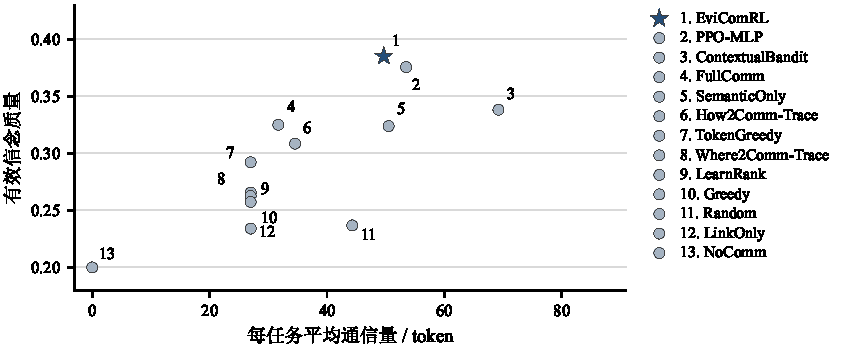
\includegraphics[width=.98\textwidth]{figures/rq2/quality_cost.pdf}
\bicaption{基准配置下的有效信念质量与每任务平均通信量}{Effective belief quality versus average token expenditure per task under the main setting}
\label{rq2:fig:tradeoff}
\end{figure}

\subsection{观测与通信条件的影响}

首先考察局部视角数量的影响（图~\ref{rq2:fig:agents}）。当局部视角从 3 个增至 6 个再增至 9 个时，准确率依次由 35.00\% 跃升至 53.83\% 和 58.17\%，宏平均 F1 亦由 22.06\% 提升至 43.33\% 和 50.58\%。其中 3 至 6 个视角阶段增益最为显著，因为多视角迅速补齐了单机视野盲区；而从 6 个增至 9 个视角时，有效信念质量由 0.3635 进一步升至 0.3854，每任务平均通信量反而从 51.08 token 微降至 49.70 token。这说明在候选池上限固定的前提下，只要前端筛选能挑出更优质的视角，增加观测节点并不必然提高通信开销，反而能让策略做出更好的选择。

\begin{figure}[htbp]
\centering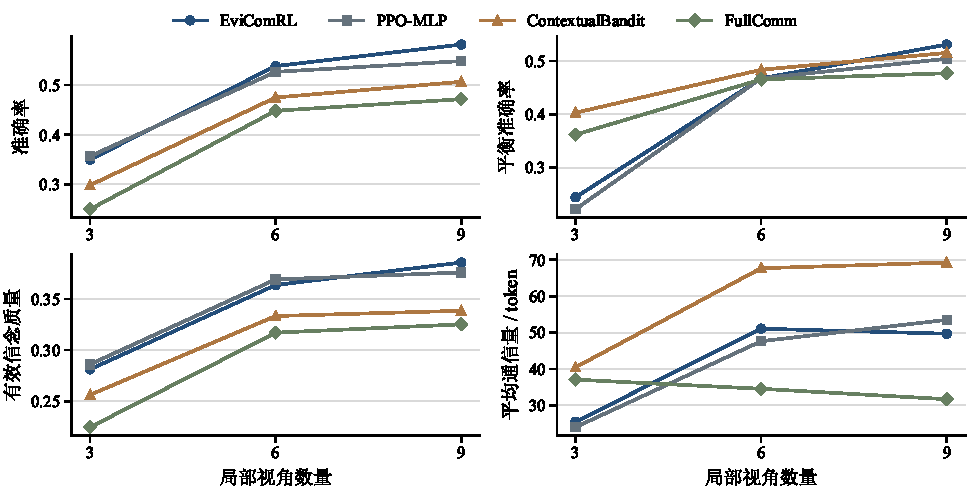
\includegraphics[width=\textwidth]{figures/rq2/agent_count.pdf}
\bicaption{不同局部视角数量下的质量与通信开销}{Quality and communication cost with different numbers of local views}
\label{rq2:fig:agents}
\end{figure}

图~\ref{rq2:fig:budget} 给出了通信预算分别设为 60、120、180 和 240 个词元时的实验结果。当预算从 60 放宽到 120 个词元时，分类准确率由 58.00\% 略升至 58.17\%，整体变化不大，但宏平均 F1 从 48.04\% 提高到 50.58\%，有效信念质量也从 0.3729 升至 0.3854，说明放宽预算后少数类别的分类效果和整体置信度均有所改善。预算继续增加到 180 和 240 个词元时，受 3 条接收容量以及主动停止的限制，策略的实际平均开销基本停留在 55.68 和 55.53 个词元，分类准确率反而小幅回落至 55.50\% 和 55.33\%。这主要是因为不同预算下的策略需要分别训练，而预算值直接参与特征归一化、候选初筛排序以及奖励中的开销缩放，从而影响了策略最终的收敛结果。

\begin{figure}[htbp]
\centering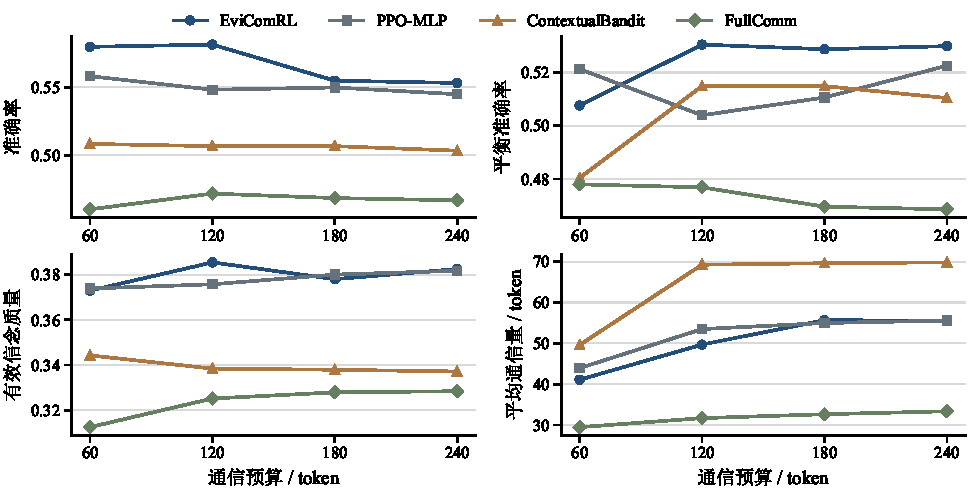
\includegraphics[width=\textwidth]{figures/rq2/budget.pdf}
\bicaption{不同通信预算下的性能变化}{Performance under different communication budgets}
\label{rq2:fig:budget}
\end{figure}

% 对应图片保留在 figures/rq2/，本稿不再引用。

图~\ref{rq2:fig:links} 对比了良好、中等和较差三种链路条件下的实验结果，对应的最低送达概率门限分别为 0.35、0.45 和 0.25，以确保较差链路下仍有可用候选。当链路条件由中等降为较差时，分类准确率仅从 58.17\% 降至 56.00\%，但有效信念质量从 0.3854 降至 0.2453，QCR 也从 0.1780 降至 0.0845。这说明仅看分类准确率容易低估链路变差的影响，即使最终分类结果尚未改变，消息送达概率和分类置信度也已经明显下降。

\begin{figure}[htbp]
\centering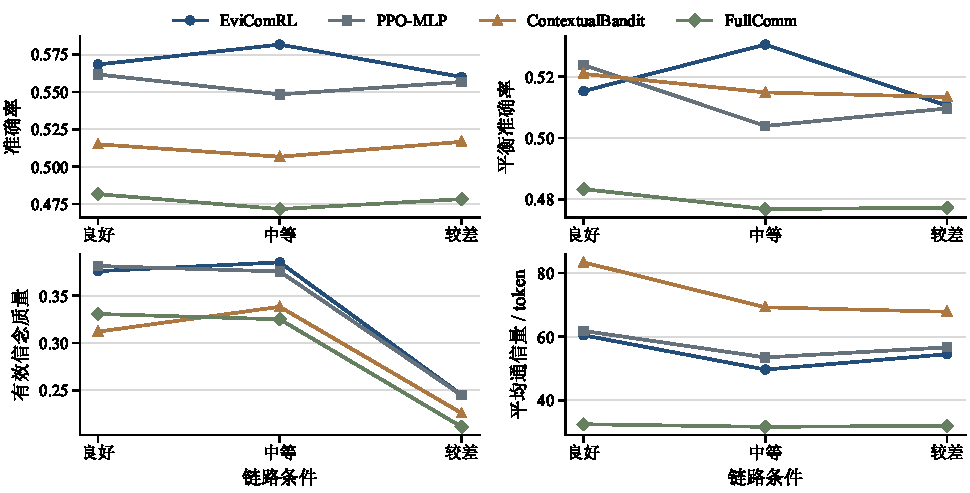
\includegraphics[width=\textwidth]{figures/rq2/link_profile.pdf}
\bicaption{不同链路条件下的推理质量与成本}{Inference quality and cost under different link conditions}
\label{rq2:fig:links}
\end{figure}

% 对应图片保留在 figures/rq2/，本稿不再引用。

此外，在消息模式开放实验中，依次放开标签、陈述、摘要与完整证据四种模式。仅允许发送短标签时，策略仅耗费 24.14 token 即取得了 57.00\% 的准确率、53.63\% 的平衡准确率及 51.26\% 的宏平均 F1；放开全部模式后，通信量增至 49.70 token，准确率略升至 58.17\%，有效信念质量从 0.3284 明显提高至 0.3854，但平衡准确率与宏平均 F1 未同步上升。原因在于五级可见性任务属于离散分类，短标签已直接包含局部类别判断，而长消息虽然融合权重更高，却伴随着更大的发送时延与丢包风险，因此表达越完整并不意味着所有分类指标都能单调提升。

\subsection{消融实验}

% 对应图片保留在 figures/rq2/，本稿不再引用。

表~\ref{rq2:tab:ablation} 给出了各主要模块的消融实验结果。移除成本敏感检索与重排序、改为直接按默认顺序截取候选池后，分类准确率从 58.17\% 降至 51.00\%，宏平均 F1 随之下降 7.07 个百分点，说明候选池质量直接影响后续选择策略的效果。仅去除重排序中的链路项时，分类准确率与宏平均 F1 分别下降 1.67 和 1.92 个百分点。去掉单步前瞻预训练后，分类准确率降至 55.00\%，同时平均每次任务的通信开销增至 55.94 个词元，说明单步前瞻预训练不仅有助于策略收敛，也能减少冗余发送并及时停止。

% 对应图片保留在 figures/rq2/，本稿不再引用。

\begin{table}[htbp]
\centering\small
\bicaption{主要消融设置的分类质量与通信代价}{Classification quality and communication cost of main ablation settings}
\label{rq2:tab:ablation}
\begin{tabular}{lrrrrr}
\toprule
设置 & Acc/\% & BAcc/\% & MF1/\% & \shortstack{每任务平均\\通信量/token} & $Q_{\mathrm{eff}}$\\
\midrule
完整方法 & 58.17 & 53.05 & 50.58 & 49.70 & 0.3854\\
取消重排序 & 51.00 & 46.39 & 43.51 & 44.48 & 0.3500\\
取消链路排序 & 56.50 & 52.16 & 48.66 & 46.66 & 0.3785\\
取消中心偏好 & 58.17 & 53.05 & 50.58 & 49.70 & 0.3854\\
取消长度代价 & 56.33 & 50.55 & 48.61 & 51.20 & 0.3766\\
取消风险代价 & 56.67 & 54.17 & 50.62 & 52.80 & 0.3815\\
取消预训练 & 55.00 & 51.41 & 48.33 & 55.94 & 0.3723\\
取消盲中心 & 27.17 & 36.41 & 25.19 & 16.90 & 0.2726\\
取消增量折扣 & 58.50 & 53.20 & 50.79 & 49.51 & 0.3957\\
\bottomrule
\end{tabular}
\end{table}

从奖励项与实验设定的消融结果来看，去掉长度代价惩罚会同时增加词元开销并降低分类性能；去掉风险代价惩罚虽然使平衡准确率略有上升，但分类准确率、有效信念质量和 QCR 均有所下降。去掉中心偏好项后，各项指标保持不变，与前文关于所有消息均发往地面中心时该常数项不影响排序的分析一致；而改为地面中心具备本地观测后，初始状态、候选消息流向与信念更新规则均会随之改变，因此该组结果不宜直接与基准配置对比。此外，取 $\alpha=0$ 去掉送达概率折扣后，分类准确率略升至 58.50\%，有效信念质量达到 0.3957，说明在当前的离线确定性融合下，平方根折扣设置偏于保守，实际部署时可根据信道条件调整折扣系数 $\alpha$。

% 对应图片保留在 figures/rq2/，本稿不再引用。

\section{本章小结}
\label{rq2:sec:summary}

本章针对有限词元预算下的冗余传输和低质量视角干扰问题，提出了语义消息选择方法 EviComRL。该方法先通过成本敏感检索与重排序缩小候选范围，再利用关系编码与上下文池化模块融合候选特征与已选历史信息，并结合单步前瞻预训练和掩码 PPO，学习消息来源、语义模式与停止时机的决策策略。实验结果表明，EviComRL 在基准配置下的分类准确率达到 58.17\%，较 FullComm 和 ContextualBandit 分别高出 11.00 和 7.50 个百分点。此外，增加局部视角能够提供更多有效信息，而单纯放宽消息长度并不总能改善各项分类指标；消融实验也验证了成本敏感检索与重排序、链路项和单步前瞻预训练对提升分类性能与降低通信开销的作用。
